\documentclass[crop,tikz]{standalone}
\usetikzlibrary{backgrounds}
\colorlet{blue}{cyan}
\tikzset{
  inverted/.style = {
    every path/.style = {draw=white,text=white},
    background rectangle/.style={fill},
    show background rectangle
  }
}

\usepackage{amsmath}
\usetikzlibrary{decorations.markings}
\tikzset{>=latex}
\colorlet{green}{green}
\newcommand{\FZf}{\vec{F}_\text{Zf}}

\begin{document}
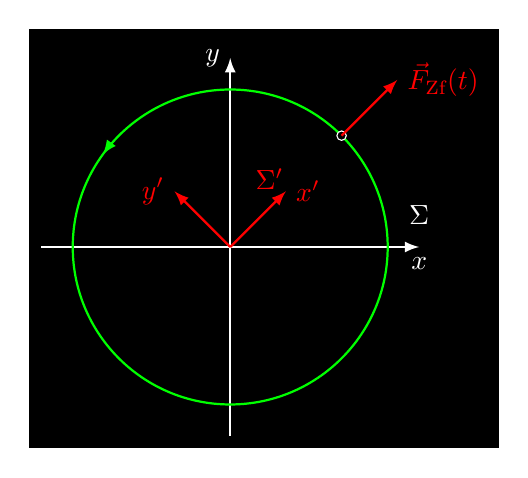
\begin{tikzpicture}[inverted,scale=2]
  \draw[->,thick] (-1.2,0) -- (1.2,0) node[below] {$x$};
  \draw[->,thick] (0,-1.2) -- (0,1.2) node[left] {$y$};
  \draw[->,red,thick] (0,0) -- (45:0.5) node[right] {$x'$};
  \draw[->,red,thick] (0,0) -- (90+45:0.5) node[left] {$y'$};
  \draw[
    decoration={markings, mark=at position 0.4 with {\arrow{>}}},
    postaction={decorate},
    green,
    thick
  ] (0,0) circle (1);
  \draw[fill] (45:1) circle (0.03);
  \draw[->,red,thick] (45:1) -- +(45:0.5) node[right]{$\FZf(t)$};
  \node at (1.2,0.2) {$\Sigma$};
  \node at (60:0.5) {\textcolor{red}{$\Sigma'$}};
\end{tikzpicture}
\end{document}
